\documentclass[14pt]{extbook}
\usepackage{multicol, enumerate, enumitem, hyperref, color, soul, setspace, parskip, fancyhdr} %General Packages
\usepackage{amssymb, amsthm, amsmath, latexsym, units, mathtools} %Math Packages
\everymath{\displaystyle} %All math in Display Style
% Packages with additional options
\usepackage[headsep=0.5cm,headheight=12pt, left=1 in,right= 1 in,top= 1 in,bottom= 1 in]{geometry}
\usepackage[usenames,dvipsnames]{xcolor}
\usepackage{dashrule}  % Package to use the command below to create lines between items
\newcommand{\litem}[1]{\item#1\hspace*{-1cm}\rule{\textwidth}{0.4pt}}
\pagestyle{fancy}
\lhead{Makeup Progress Quiz 2}
\chead{}
\rhead{Version C}
\lfoot{5763-3522}
\cfoot{}
\rfoot{Spring 2021}
\begin{document}

\begin{enumerate}
\litem{
Solve the rational equation below. Then, choose the interval(s) that the solution(s) belongs to.\[ \frac{-16}{16x -48} + 1 = \frac{-16}{16x -48} \]\begin{enumerate}[label=\Alph*.]
\item \( x_1 \in [2, 5] \text{ and } x_2 \in [3,5] \)
\item \( x_1 \in [-3, -1] \text{ and } x_2 \in [3,5] \)
\item \( x \in [3.0,4.0] \)
\item \( x \in [-3,-1] \)
\item \( \text{All solutions lead to invalid or complex values in the equation.} \)

\end{enumerate} }
\litem{
Determine the domain of the function below.\[ f(x) = \frac{4}{20x^{2} +9 x -18} \]\begin{enumerate}[label=\Alph*.]
\item \( \text{All Real numbers except } x = a, \text{ where } a \in [-2.2, -0.2] \)
\item \( \text{All Real numbers.} \)
\item \( \text{All Real numbers except } x = a \text{ and } x = b, \text{ where } a \in [-2.2, -0.2] \text{ and } b \in [0.75, 1.75] \)
\item \( \text{All Real numbers except } x = a, \text{ where } a \in [-32, -27] \)
\item \( \text{All Real numbers except } x = a \text{ and } x = b, \text{ where } a \in [-32, -27] \text{ and } b \in [10, 15] \)

\end{enumerate} }
\litem{
Choose the equation of the function graphed below.
\begin{center}
    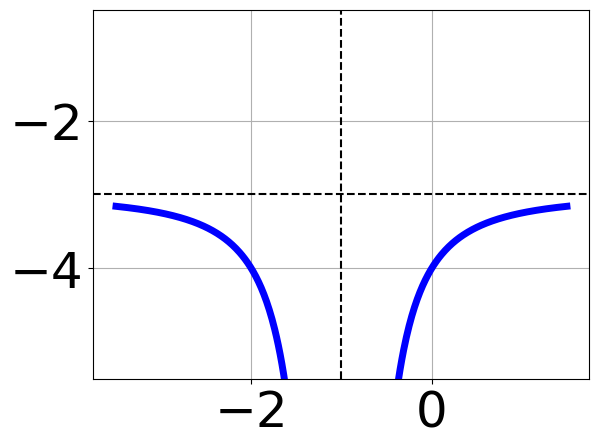
\includegraphics[width=0.5\textwidth]{../Figures/rationalGraphToEquationCopyC.png}
\end{center}
\begin{enumerate}[label=\Alph*.]
\item \( f(x) = \frac{-1}{(x + 1)^2} - 3 \)
\item \( f(x) = \frac{1}{(x - 1)^2} - 3 \)
\item \( f(x) = \frac{-1}{x + 1} - 3 \)
\item \( f(x) = \frac{1}{x - 1} - 3 \)
\item \( \text{None of the above} \)

\end{enumerate} }
\litem{
Choose the equation of the function graphed below.
\begin{center}
    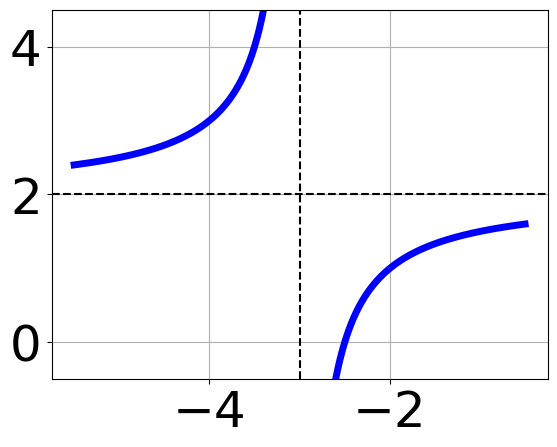
\includegraphics[width=0.5\textwidth]{../Figures/rationalGraphToEquationC.png}
\end{center}
\begin{enumerate}[label=\Alph*.]
\item \( f(x) = \frac{-1}{x - 3} + 2 \)
\item \( f(x) = \frac{1}{(x + 3)^2} + 2 \)
\item \( f(x) = \frac{1}{x + 3} + 2 \)
\item \( f(x) = \frac{-1}{(x - 3)^2} + 2 \)
\item \( \text{None of the above} \)

\end{enumerate} }
\litem{
Solve the rational equation below. Then, choose the interval(s) that the solution(s) belongs to.\[ \frac{-4x}{2x + 2} + \frac{-7x^{2}}{8x^{2} -2 x -10} = \frac{-4}{4x -5} \]\begin{enumerate}[label=\Alph*.]
\item \( x_1 \in [-0.28, -0.05] \text{ and } x_2 \in [0.4,2.6] \)
\item \( \text{All solutions lead to invalid or complex values in the equation.} \)
\item \( x \in [1.01,1.25] \)
\item \( x_1 \in [-0.28, -0.05] \text{ and } x_2 \in [-2.6,-0.4] \)
\item \( x \in [1.42,1.57] \)

\end{enumerate} }
\litem{
Solve the rational equation below. Then, choose the interval(s) that the solution(s) belongs to.\[ \frac{126}{28x + 42} + 1 = \frac{126}{28x + 42} \]\begin{enumerate}[label=\Alph*.]
\item \( x \in [0.5,2.5] \)
\item \( x_1 \in [-1.5, -0.5] \text{ and } x_2 \in [1.5,3.5] \)
\item \( \text{All solutions lead to invalid or complex values in the equation.} \)
\item \( x_1 \in [-1.5, -0.5] \text{ and } x_2 \in [-1.5,0.5] \)
\item \( x \in [-1.5,1.5] \)

\end{enumerate} }
\litem{
Determine the domain of the function below.\[ f(x) = \frac{5}{24x^{2} -56 x + 30} \]\begin{enumerate}[label=\Alph*.]
\item \( \text{All Real numbers except } x = a \text{ and } x = b, \text{ where } a \in [0.69, 1.28] \text{ and } b \in [1.49, 1.83] \)
\item \( \text{All Real numbers except } x = a, \text{ where } a \in [0.69, 1.28] \)
\item \( \text{All Real numbers except } x = a \text{ and } x = b, \text{ where } a \in [23.24, 24.27] \text{ and } b \in [29.78, 30.32] \)
\item \( \text{All Real numbers except } x = a, \text{ where } a \in [23.24, 24.27] \)
\item \( \text{All Real numbers.} \)

\end{enumerate} }
\litem{
Choose the graph of the equation below.\[ f(x) = \frac{1}{(x + 1)^2} + 2 \]\begin{enumerate}[label=\Alph*.]
\begin{multicols}{2}\item 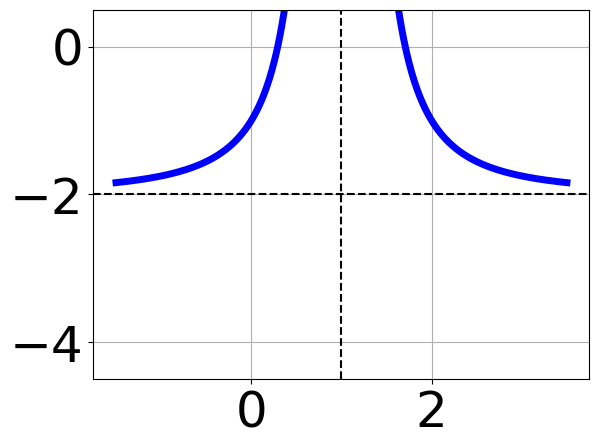
\includegraphics[width = 0.3\textwidth]{../Figures/rationalEquationToGraphCopyAC.png}\item 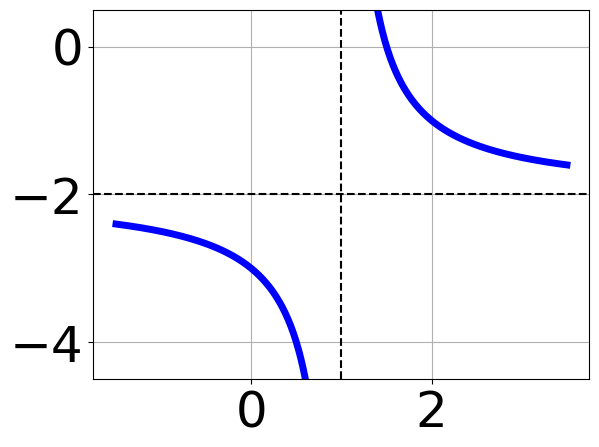
\includegraphics[width = 0.3\textwidth]{../Figures/rationalEquationToGraphCopyBC.png}\item 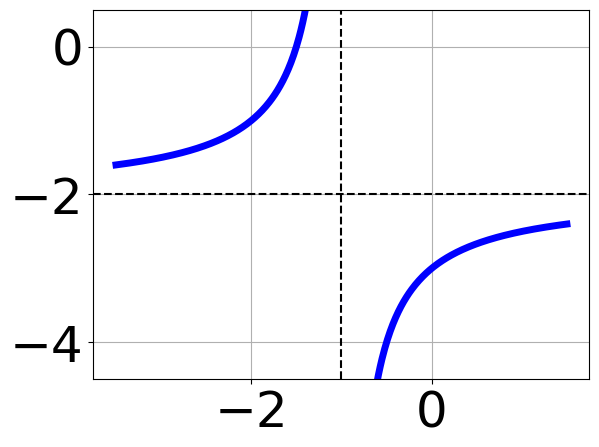
\includegraphics[width = 0.3\textwidth]{../Figures/rationalEquationToGraphCopyCC.png}\item 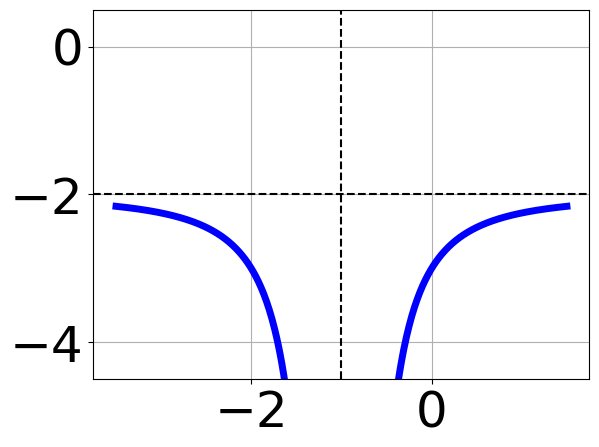
\includegraphics[width = 0.3\textwidth]{../Figures/rationalEquationToGraphCopyDC.png}\end{multicols}\item None of the above.
\end{enumerate} }
\litem{
Choose the graph of the equation below.\[ f(x) = \frac{-1}{(x + 1)^2} + 3 \]\begin{enumerate}[label=\Alph*.]
\begin{multicols}{2}\item 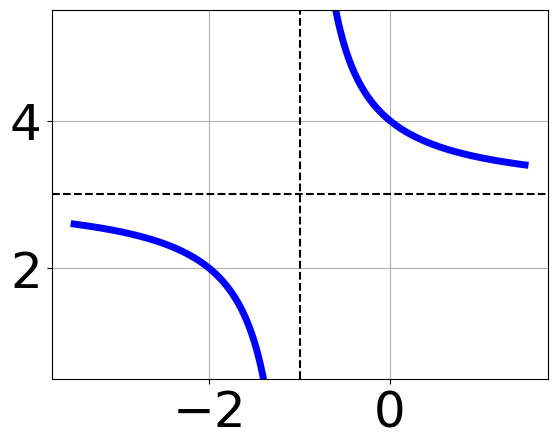
\includegraphics[width = 0.3\textwidth]{../Figures/rationalEquationToGraphAC.png}\item 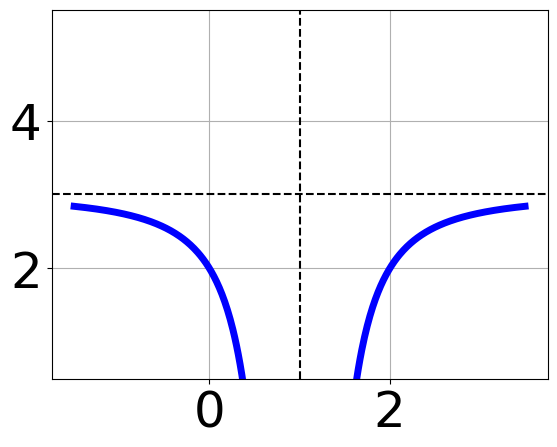
\includegraphics[width = 0.3\textwidth]{../Figures/rationalEquationToGraphBC.png}\item 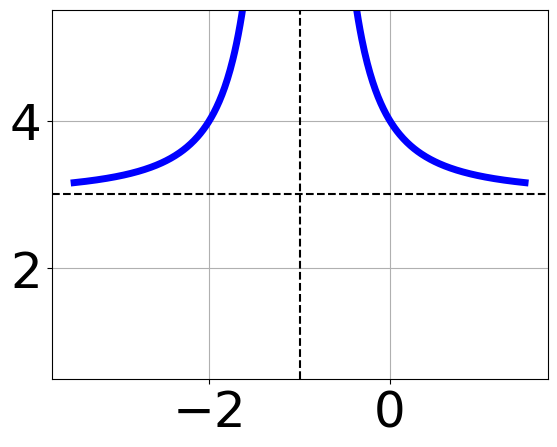
\includegraphics[width = 0.3\textwidth]{../Figures/rationalEquationToGraphCC.png}\item 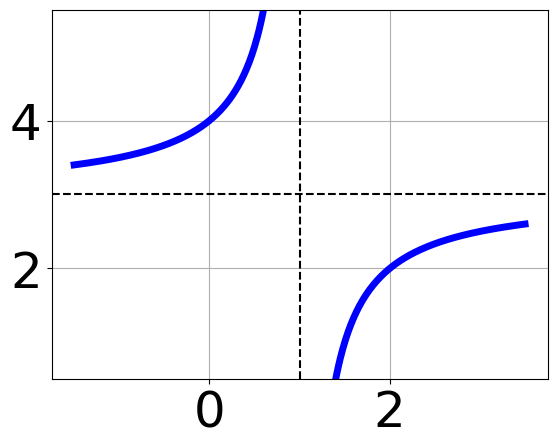
\includegraphics[width = 0.3\textwidth]{../Figures/rationalEquationToGraphDC.png}\end{multicols}\item None of the above.
\end{enumerate} }
\litem{
Solve the rational equation below. Then, choose the interval(s) that the solution(s) belongs to.\[ \frac{-5x}{-4x -6} + \frac{-2x^{2}}{16x^{2} +40 x + 24} = \frac{-6}{-4x -4} \]\begin{enumerate}[label=\Alph*.]
\item \( x_1 \in [-1.44, -1.06] \text{ and } x_2 \in [-3.5,1.5] \)
\item \( x \in [-1.07,-0.22] \)
\item \( x_1 \in [-1.44, -1.06] \text{ and } x_2 \in [1.53,2.53] \)
\item \( \text{All solutions lead to invalid or complex values in the equation.} \)
\item \( x \in [0.79,1.78] \)

\end{enumerate} }
\end{enumerate}

\end{document}